% \documentclass{article}
% \documentclass{book}
\documentclass{report} % Chọn cỡ chữ
\usepackage{Start}
\begin{document} % Bắt đầu
%!%%%%%%%%%%%%%%%%%%%%%%%%%%%%
%!%%%%%%%%%%%%%%%%%%%%%%%%%%%%
%!%%%%%%%%%%%%%%%%%%%%%%%%%%%%
%!%%%%%%%%%%%%%%%%%%%%%%%%%%%%
%!%%%%%%%%%%%%%%%%%%%%%%%%%%%%
%!%%%%%%%%%%%%%%%%%%%%%%%%%%%%
%!%%%%%%%%%%%%%%%%%%%%%%%%%%%%
%!%%%%%%%%%%%%%%%%%%%%%%%%%%%%
%!%%%%%%%%%%%%%%%%%%%%%%%%%%%%
%!%%%%%%%%%%%%%%%%%%%%%%%%%%%%
%!%%%%%%%%%%%%%%%%%%%%%%%%%%%%
%!%%%%%%%%%%%%%%%%%%%%%%%%%%%%
%!%%%%%%%%%%%%%%%%%%%%%%%%%%%%
%!%%%%%%%%%%%%%%%%%%%%%%%%%%%%
%!%%%%%%%%%%%%%%%%%%%%%%%%%%%%
%!%%%%%%%%%%%%%%%%%%%%%%%%%%%%
%!%%%%%%%%%%%%%%%%%%%%%%%%%%%%
%!%%%%%%%%%%%%%%%%%%%%%%%%%%%%
%!%%%%%%%%%%%%%%%%%%%%%%%%%%%%
%!%%%%%%%%%%%%%%%%%%%%%%%%%%%%
%!%%%%%%%%%%%%%%%%%%%%%%%%%%%%
%!%%%%%%%%%%%%%%%%%%%%%%%%%%%%
%!%%%%%%%%%%%%%%%%%%%%%%%%%%%%
%!%%%%%%%%%%%%%%%%%%%%%%%%%%%%
%!%%%%%%%%%%%%%%%%%%%%%%%%%%%%
%!%%%%%%%%%%%%%%%%%%%%%%%%%%%%
%# Phần đầu
%#%%%%%%%%%%%%%%%%%%%%%%%%%%%%
% \begin{titlepage}

    % Vẽ hình chữ nhật
    
    \begin{tikzpicture}[remember picture, overlay]\draw [line width = 3pt]($ (current page.north west) + (3.0cm, - 2.5cm)$)rectangle($ (current page.south east) + (- 2.5cm, 2.5cm)$);\draw [line width = 0.5pt]($ (current page.north west) + (3.1cm, - 2.6cm)$)rectangle($ (current page.south east) + (- 2.6cm, 2.6cm)$);\end{tikzpicture}
    
    \begin{center}
    
    \vspace{- 0.4cm}
    
    \textbf{ĐẠI HỌC BÁCH KHOA HÀ NỘI} \\
    
    \textbf{VIỆN TOÁN ỨNG DỤNG VÀ TIN HỌC} \\
    
    \textbf{******}
    
    \vspace{0.8cm}
    
    \begin{figure}[H]
    
    \centering
    
    
\includegraphics[scale = 0.5]{pictures/_hust/main.png}
    
    \end{figure}
    
    \vspace{0.7cm}
    
    \textbf{\fontsize{16pt}{30pt}\selectfont {BÁO CÁO ĐỒ ÁN II}}
    
    \vspace{1cm}
    
    \textbf{\fontsize{16pt}{30pt}\selectfont {ĐỀ TÀI:}} \\
    
    \textbf{\fontsize{20pt}{24pt}\selectfont {Sử dụng thiết kế hướng miền \\ xây dựng kiến trúc vi dịch vụ cho \\ bài toán hóa đơn điện tử}} \\
    
    \end{center}
    
    \vspace{0.3cm}
    
    \begin{center}
    
    \textbf{\fontsize{10pt}{24pt}\selectfont {Chuyên ngành: Toán Tin}}
    
    \end{center}
    
    \vspace{0.7cm}
    
    \hspace{3cm}\begin{minipage}{0.7\textwidth}
    
    \begin{tabular}{l l l}
    
    \textbf{\fontsize{10pt}{24pt}\selectfont {Giảng viên hướng dẫn}} & \textbf{\fontsize{10pt}{24pt}\selectfont {TS. Vũ Thành Nam}} \\
    
    \textbf{\fontsize{10pt}{24pt}\selectfont {Sinh viên thực hiện}} & \textbf{\fontsize{10pt}{24pt}\selectfont {Vũ Văn Nghĩa}} \\
    
    \textbf{\fontsize{10pt}{24pt}\selectfont {Mã số sinh viên}} & \textbf{\fontsize{10pt}{24pt}\selectfont {20206205}} \\
    
    \textbf{\fontsize{10pt}{24pt}\selectfont {Lớp}} & \textbf{\fontsize{10pt}{24pt}\selectfont {Toán Tin 02 - K65}} \\
    
    \end{tabular}
    
    \end{minipage}
    
    \vfill
    
    \begin{center}
    
    \textbf{Hà Nội, \the\year}
    
    % \textbf{Hà Nội, \the\month~/~\the\year}
    
    % \textbf{Hà Nội, \the\month~-~\the\year}
    
    \end{center}
    
    \end{titlepage}
    
    
% \begin{titlepage}

    % Vẽ hình chữ nhật
    
    \begin{tikzpicture}[remember picture, overlay]\draw [line width = 3pt]($ (current page.north west) + (3.0cm, - 2.5cm)$)rectangle($ (current page.south east) + (- 2.5cm, 2.5cm)$);\draw [line width = 0.5pt]($ (current page.north west) + (3.1cm, - 2.6cm)$)rectangle($ (current page.south east) + (- 2.6cm, 2.6cm)$);\end{tikzpicture}
    
    \begin{center}
    
    \vspace{- 0.4cm}
    
    \textbf{ĐẠI HỌC BÁCH KHOA HÀ NỘI} \\
    
    \textbf{VIỆN TOÁN ỨNG DỤNG VÀ TIN HỌC} \\
    
    \textbf{******}
    
    \vspace{0.8cm}
    
    \begin{figure}[H]
    
    \centering
    
    
\includegraphics[scale = 0.5]{pictures/_hust/main.png}
    
    \end{figure}
    
    \vspace{0.7cm}
    
    \textbf{\fontsize{16pt}{30pt}\selectfont {BÁO CÁO ĐỒ ÁN II}}
    
    \vspace{1cm}
    
    \textbf{\fontsize{16pt}{30pt}\selectfont {ĐỀ TÀI:}} \\
    
    \textbf{\fontsize{20pt}{24pt}\selectfont {Sử dụng thiết kế hướng miền \\ xây dựng kiến trúc vi dịch vụ cho \\ bài toán hóa đơn điện tử}} \\
    
    \end{center}
    
    \vspace{0.3cm}
    
    \begin{center}
    
    \textbf{\fontsize{10pt}{24pt}\selectfont {Chuyên ngành: Toán Tin}}
    
    \end{center}
    
    \vspace{0.7cm}
    
    \hspace{3cm}\begin{minipage}{0.7\textwidth}
    
    \begin{tabular}{l l l}
    
    \textbf{\fontsize{10pt}{24pt}\selectfont {Giảng viên hướng dẫn}} & \textbf{\fontsize{10pt}{24pt}\selectfont {TS. Vũ Thành Nam}} \\
    
    \textbf{\fontsize{10pt}{24pt}\selectfont {Sinh viên thực hiện}} & \textbf{\fontsize{10pt}{24pt}\selectfont {Vũ Văn Nghĩa}} \\
    
    \textbf{\fontsize{10pt}{24pt}\selectfont {Mã số sinh viên}} & \textbf{\fontsize{10pt}{24pt}\selectfont {20206205}} \\
    
    \textbf{\fontsize{10pt}{24pt}\selectfont {Lớp}} & \textbf{\fontsize{10pt}{24pt}\selectfont {Toán Tin 02 - K65}} \\
    
    \end{tabular}
    
    \end{minipage}
    
    \vfill
    
    \begin{center}
    
    \textbf{Hà Nội, \the\year}
    
    % \textbf{Hà Nội, \the\month~/~\the\year}
    
    % \textbf{Hà Nội, \the\month~-~\the\year}
    
    \end{center}
    
    \end{titlepage}
    
    
% \begin{center}

    {\bfseries NHẬN XÉT CỦA GIẢNG VIÊN HƯỚNG DẪN}
    
    \end{center}
    
    \begin{enumerate}
    
    \item Mục đích và nội dung của đồ án:
    
    \vspace{20ex}
    
    \item Kết quả đạt được:
    
    \vspace{20ex}
    
    \item Ý thức làm việc của sinh viên:
    
    \vspace{20ex}
    
    \end{enumerate}
    
    \hspace{0.4\textwidth}\begin{minipage}{0.5\textwidth}
    
    \noindent\begin{center}
    
    \textit{Hà Nội, \today} \\
    
    \textbf{Giảng viên hướng dẫn} \\
    
    \textit{(Ký và ghi rõ họ tên)}
    
    \vspace{2cm}
    
    \textbf{TS. Vũ Thành Nam}
    
    \end{center}
    
    \end{minipage}
    
    \pagestyle{empty}
    
    
% 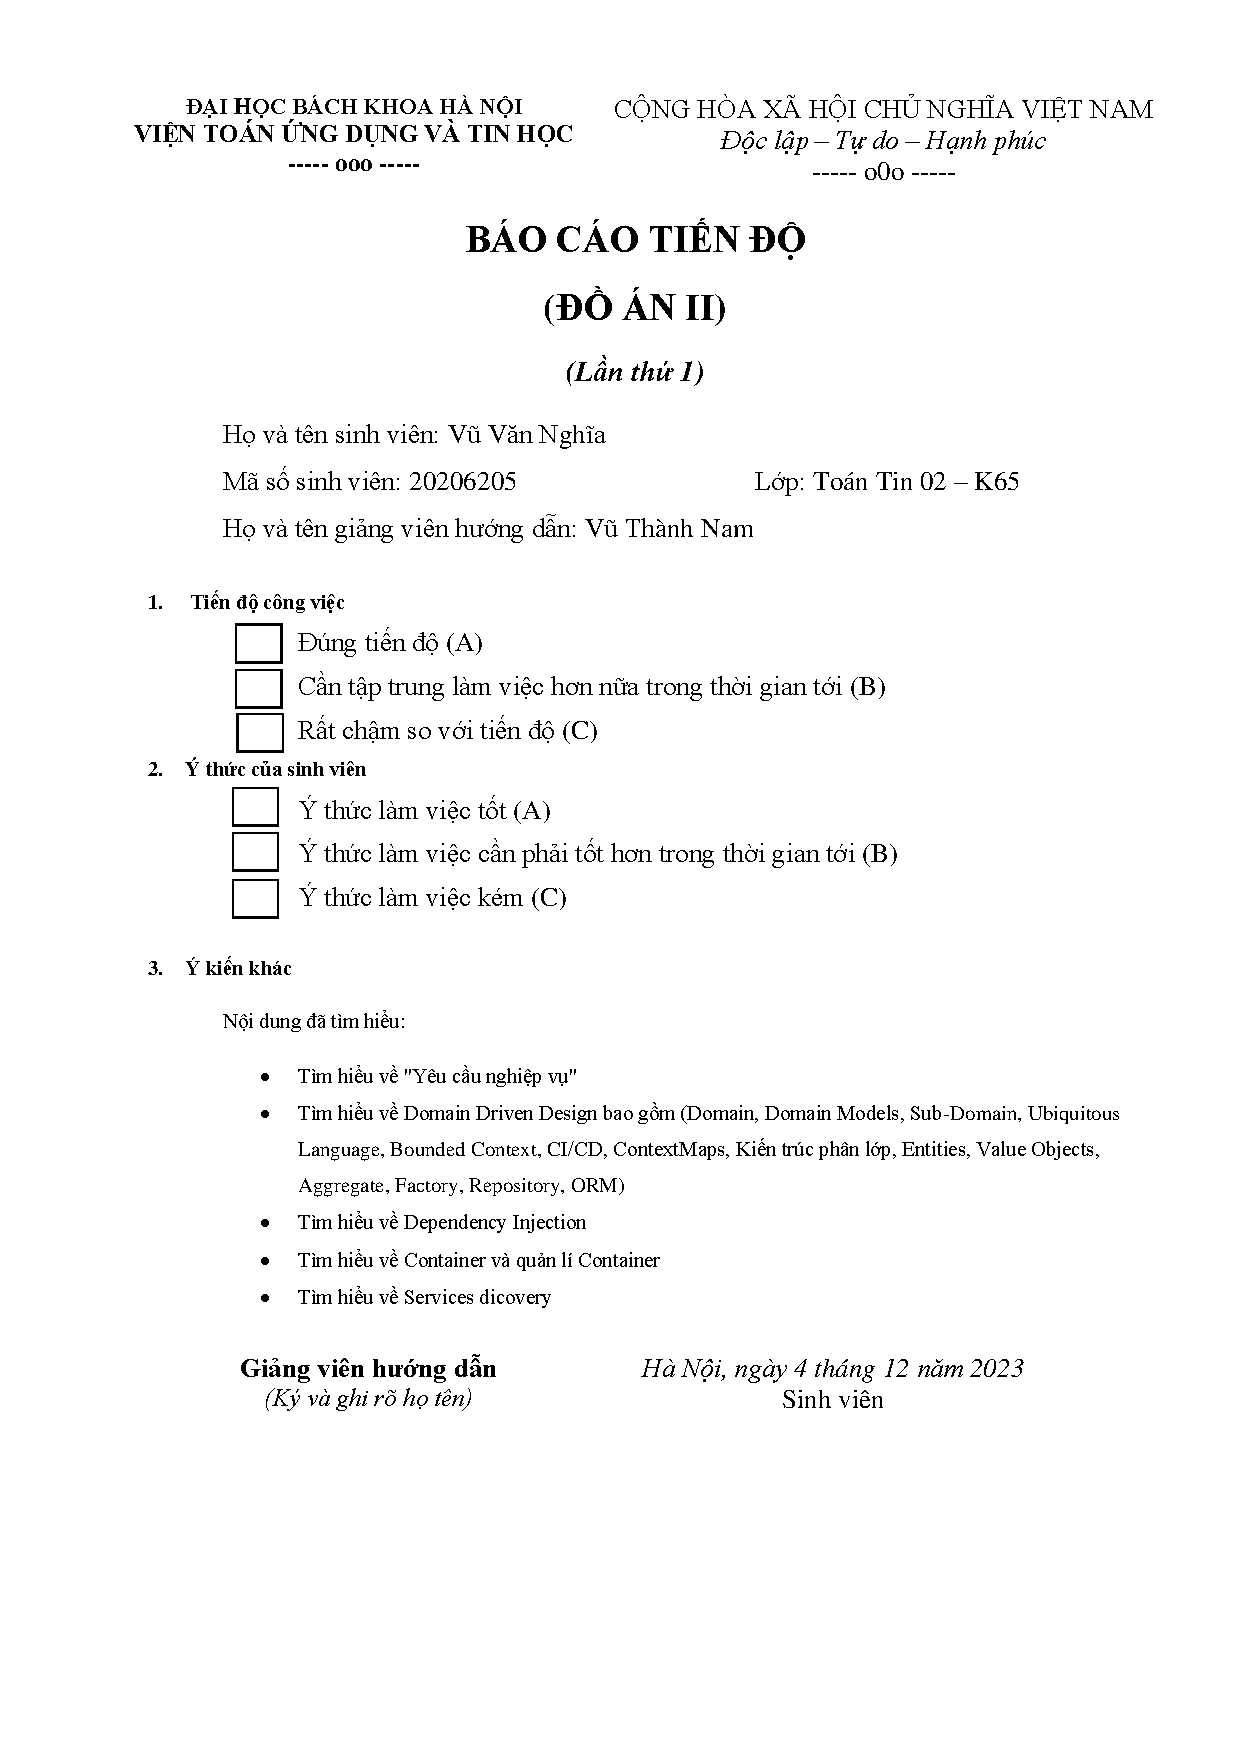
\includepdf[pages = -]{contents/bao_cao_tien_do/lan_1.pdf}
% 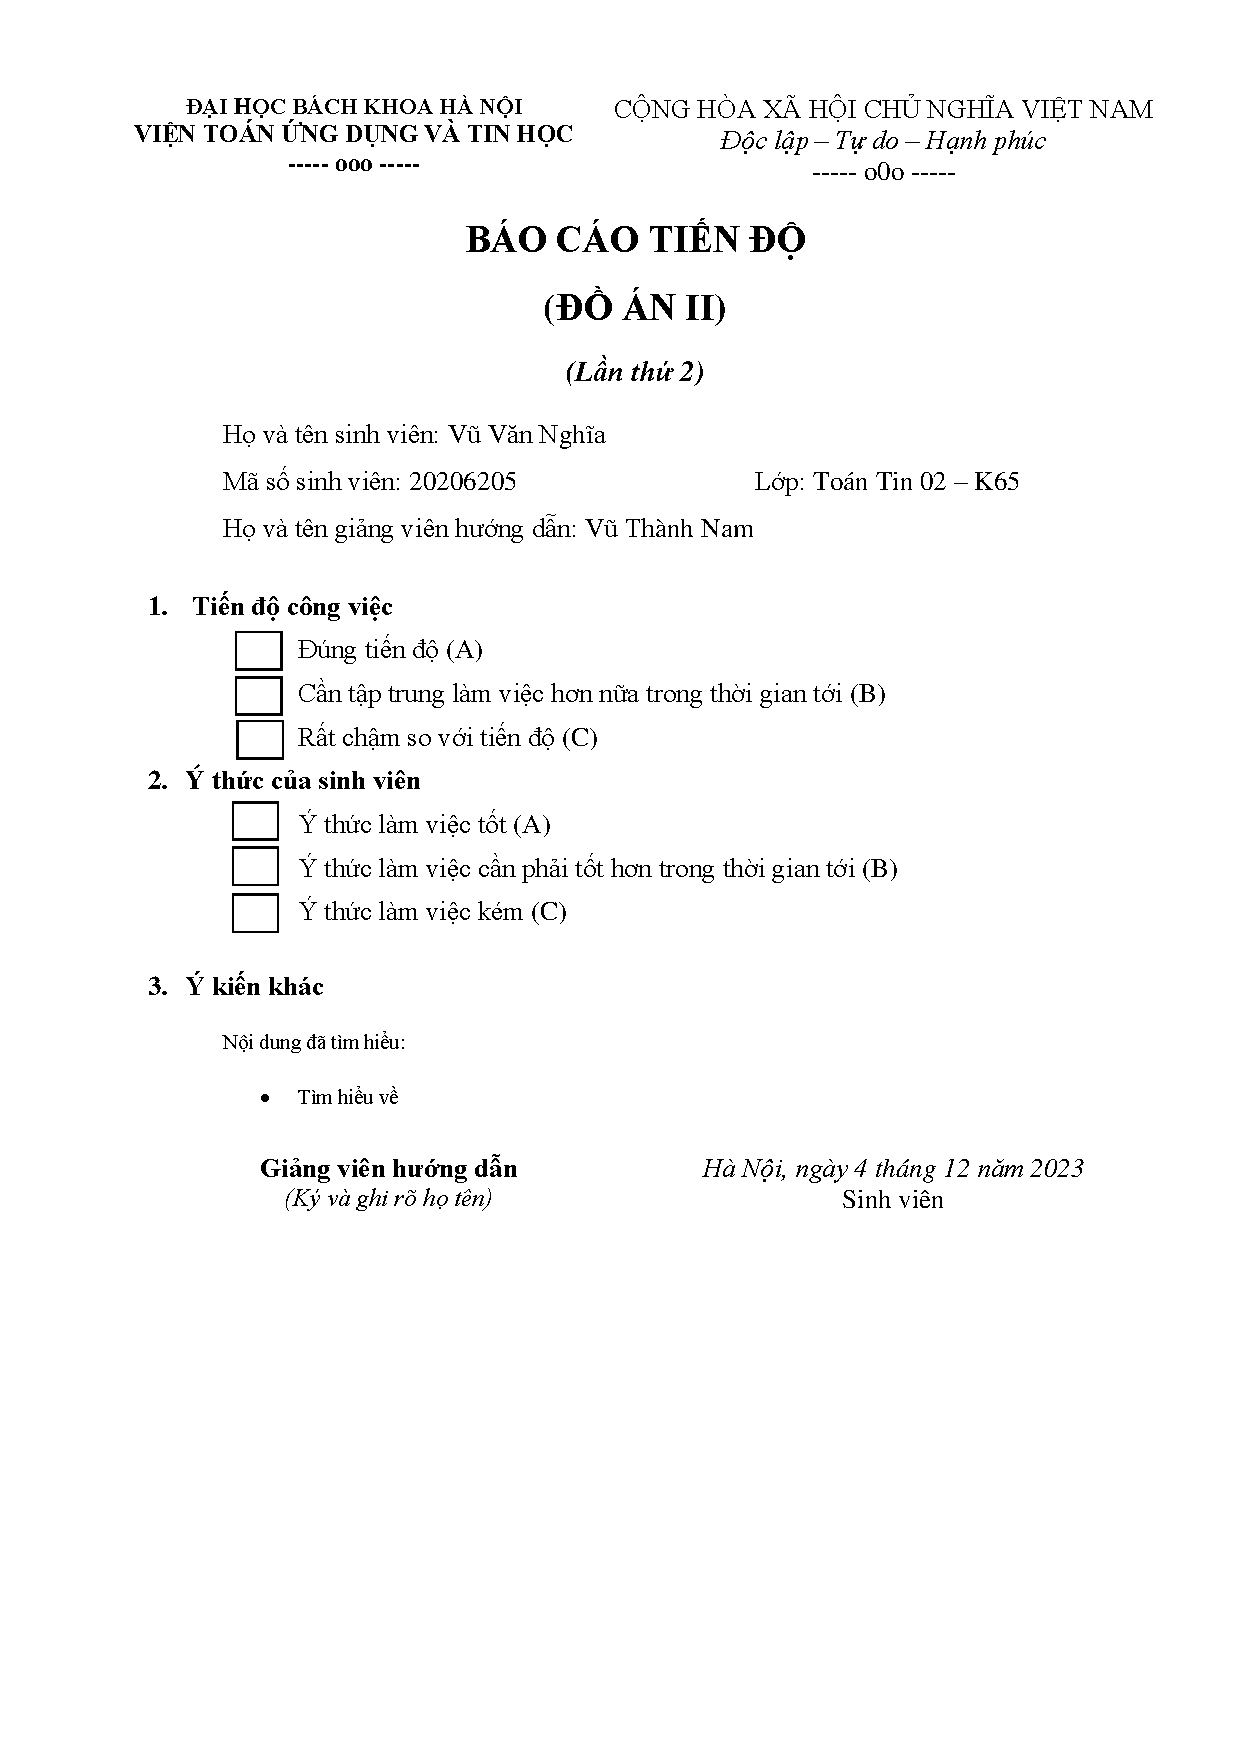
\includepdf[pages = -]{contents/bao_cao_tien_do/lan_2.pdf}
% \renewcommand*\contentsname{\centering MỤC LỤC}

\tableofcontents

\setcounter{page}{0}


% \chapter*{\centering LỜI CẢM ƠN}

\addcontentsline{toc}{chapter}{LỜI CẢM ƠN}

Trước hết, em xin gửi lời cảm ơn chân thành và sâu sắc đến TS. Vũ Thành Nam, người thầy đã tận tình hỗ trợ và hướng dẫn em suốt thời gian thực hiện đồ án. Những kiến thức và kinh nghiệm mà em đã tiếp thu được trong quá trình này sẽ đóng góp quan trọng vào sự phát triển và thành công của em trong tương lai. Em xin gửi lời chúc sức khỏe tốt nhất đến thầy, hy vọng thầy luôn dồi dào sức khỏe, đam mê và nhiệt huyết trong công việc giảng dạy.

Em cũng xin gửi lời cảm ơn tới các thầy cô giảng viên trong \emph{"Khoa Toán - Tin"} đã tận tình truyền đạt những kiến thức quý báu cho em. Những kiến thức này không chỉ giúp em phát triển về mặt tri thức mà còn nuôi dưỡng kỹ năng và đam mê trong quá trình học tập và nghiên cứu.

Trong quá trình hoàn thành bài báo cáo đồ án này không tránh khỏi những thiếu sót. Vì vậy, em mong nhận được sự giúp đỡ và ý kiến đóng góp chân thành từ các thầy cô để em có thể cải thiện một cách tốt nhất.

\emph{Em xin chân thành cảm ơn!}

\vspace{0.7cm}

\hspace{0.4\textwidth}\begin{minipage}{0.5\textwidth}

\noindent\begin{center}

\textit{Hà Nội, \today} \\

\vspace{0.5cm}

\textbf{Tác giả} \\

\vspace{0.5cm}

\textbf{Vũ Văn Nghĩa}

\end{center}

\end{minipage}
% \chapter*{\centering DANH SÁCH BẢNG}

\addcontentsline{toc}{chapter}{DANH SÁCH BẢNG}

\makeatletter

\renewcommand\listoftables{

\@starttoc{lot}

}

\makeatother

\listoftables
% \chapter*{\centering DANH SÁCH HÌNH ẢNH}

\addcontentsline{toc}{chapter}{DANH SÁCH HÌNH ẢNH}

\makeatletter

\renewcommand\listoffigures{

\@starttoc{lof}

}

\makeatother

\listoffigures
% %%%%%%%%%%%%%%%%%%%%%%%%%%%%%%

%%%%%%%%%%%%%%%%%%%%%%%%%%%%%%

\chapter*{\centering DANH SÁCH CÁC CỤM TỪ VIẾT TẮT}

\addcontentsline{toc}{chapter}{DANH SÁCH CÁC CỤM TỪ VIẾT TẮT}

% @sau

% @sau

% @sau

% @sau

% @sau

% @sau

% @sau

% @sau

% @sau

% @sau

% @sau

% @sau

% @sau

% @sau

% @sau

% @sau

% @sau

% @sau

% @sau

% @sau

% @sau

% @sau

% @sau

% @sau

% @sau

% @sau

% @sau

% @sau

% @sau

% @sau

\begin{table}[h]

\centering

\begin{tabular}{|c|c|c|c|}

\hline

STT & Từ viết tắt & Từ viết đầy đủ & Mô tả \\

\hline

Dong1 & Dong1 & Cot1 & Cot2 \\

\hline

Dong2 & Dong2 & Cot1 & Cot2 \\

\hline

\end{tabular}

\end{table}

% API; Application Programming Interface; Giao diện lập trình ứng dụng

% CI/CD; Continuous Integration (CI) and Continuous Delivery (CD) ; Quá trình tích hợp và chuyển giao liên tục

% thiết kế hướng miền ; thiết kế hướng miền; Kỹ thuật thiết kế theo hướng miền

% DI; Dependency Injection; Cơ chế tiêm sự phụ thuộc giữa các đối tượng

% HTTP; Hypertext Transfer Protocol; Giao thức truyền tải siêu văn bản

% JSON; JavaScript Object Notation; Một kiểu dữ liệu mở rộng của JavaScript

% ORM; Object Relational Mapping; Một kỹ thuật ánh xạ các đối tượng lập trình với từng bảng trong CSDL quan hệ

% Cơ sở dữ liệu ; CSDL ;

% Tạo (Create), Đọc (Read), Sửa (Update), Xóa (Delete) ; CRUD ;

% Kubernetes ; K8s ; kubernetes

% Số điện thoại ; SĐT ;

% UML

% MVC; Model View Controller; Một mẫu thiết kế ứng dụng

% SQL

SOA; Service Oriented Architecture; Kiến trúc hướng dịch vụ

SOAP; Simple Object Access Protocol; Một giao thức để truy cập dịch vụ web

SPA; Single Page Application; Kiểu ứng dụng một trang

REST; Representational State Transfer; Một tiêu chuẩn thiết kế các API sử dụng cho các dịch vụ web

URL; Uniform Resource Locator ; Địa chỉ định vị tài nguyên trên Internet

XML; Extensible Markup Language; Ngôn ngữ đánh dấu mở rộng

% TCT ; TCT ;

Người nộp thuế ; NNT ;

Mã số thuế ; MST ;

Hóa đơn điện tử ; HĐĐT ;

Cơ quan thuế ; CQT ;

Công nghệ thông tin ; CNTT ;

%%%%%%%%%%%%%%%%%%%%%%%%%%%%%%
% \chapter*{\centering DANH SÁCH CÁC THUẬT NGỮ}

\addcontentsline{toc}{chapter}{DANH SÁCH CÁC THUẬT NGỮ}

% @sau

% @sau

% @sau

% @sau

% @sau

% @sau

% @sau

% @sau

% @sau

% @sau

% @sau

% @sau

% @sau

% @sau

% @sau

% @sau

% @sau

% @sau

% @sau

% @sau

% @sau

% @sau

% @sau

% @sau

% @sau

% @sau

% @sau

% @sau

\begin{table}[h]

\centering

\begin{tabular}{|c|c|c|}

\hline

STT & Tiếng Anh & Tiếng Việt \\

\hline

Dong1 & Dong1 & Cot2 \\

\hline

Dong2 & Dong2 & Cot2 \\

\hline

\end{tabular}

\end{table}

% kiến trúc nguyên khối, kiến trúc nguyên khối

% kiến trúc nguyên khối, kiến trúc nguyên khối

% kiến trúc vi dịch, kiến trúc vi dịch

% kiến trúc vi dịch, kiến trúc vi dịch

% kiến trúc vi dịch, kiến trúc vi dịch

% kiến trúc vi dịch, kiến trúc vi dịch

% thiết kế hướng miền, thiết kế hướng miền

% thiết kế hướng miền, thiết kế hướng miền

1 thiết kế hướng miền

Thiết kế hướng lĩnh vực

2 Domain (không dịch)

3 Abstraction Trừu tượng

4 chuyên gia ngành
%#%%%%%%%%%%%%%%%%%%%%%%%%%%%%
%%%%%%%%%%%%%%%%%%%%%%%%%%%%%%
%%%%%%%%%%%%%%%%%%%%%%%%%%%%%%
%%%%%%%%%%%%%%%%%%%%%%%%%%%%%%
%%%%%%%%%%%%%%%%%%%%%%%%%%%%%%
%%%%%%%%%%%%%%%%%%%%%%%%%%%%%%
%%%%%%%%%%%%%%%%%%%%%%%%%%%%%%
%%%%%%%%%%%%%%%%%%%%%%%%%%%%%%
%%%%%%%%%%%%%%%%%%%%%%%%%%%%%%
%%%%%%%%%%%%%%%%%%%%%%%%%%%%%%
%# Phần mở đầu đồ án nào cũng có
%#%%%%%%%%%%%%%%%%%%%%%%%%%%%%
% \chapter*{\centering MỞ ĐẦU}
% \addcontentsline{toc}{chapter}{MỞ ĐẦU}
% \section*{Lý do chọn đề tài}
% Trong quá trình hoạt động kinh doanh, doanh nghiệp có nhu cầu chuyển đổi mô hình kinh doanh linh hoạt để có thể tồn tại và phát triển khi thị trường thay đổi. Từ đó, đáp ứng nhu cầu của khách hàng, mang lại ưu thế cạnh tranh so với các đối thủ.

Trong những năm gần đây, việc áp dụng kiến trúc vi dịch vụ ngày càng phổ biến, đem lại nhiều lợi ích như tách các nghiệp vụ kinh doanh thành các dịch vụ nhỏ độc lập, tăng tính linh hoạt và khả năng chống chịu sự cố của hệ thống.

Kiến trúc vi dịch vụ hỗ trợ doanh nghiệp chuyển đổi nhanh chóng để đáp ứng nhu cầu của mô hình kinh doanh và mong đợi của khách hàng. Tuy nhiên, để xây dựng được kiến trúc vi dịch vụ tốt, cần phải tạo ra các dịch vụ nhỏ phù hợp và duy trì tính độc lập. Trong đồ án này, em sử dụng thiết kế hướng miền để phân tích và xây dựng kiến trúc vi dịch vụ.

Theo quy định của Nghị định 123/2020/NĐ - CP, tất cả các doanh nghiệp, tổ chức và hộ kinh doanh đều bắt buộc phải sử dụng hóa điện tử. Vì vậy, nhu cầu sử dụng và xử lý hóa đơn điện tử trở nên rất lớn. Do đó trong đồ án này, em chọn chủ đề \emph{"Sử dụng thiết kế hướng miền xây dựng kiến trúc vi dịch vụ cho bài toán hóa đơn điện tử"}. Chủ đề này là một xu hướng quan trọng trong phát triển phần mềm và mang lại nhiều lợi ích trong việc cải thiện quá trình quản lý hóa đơn điện tử.
% \section*{Đối tượng và phạm vi nghiên cứu}
% \begin{itemize}

\item \textbf{Đối tượng nghiên cứu:} Kiến trúc vi dịch vụ

\item \textbf{Phạm vi nghiên cứu:} Tập trung vào tìm hiểu thiết kế hướng miền xây dựng kiến trúc vi dịch vụ cho bài toán hóa đơn điện tử.

\end{itemize}


% \section*{Tóm tắt nội dung đồ án}
% Báo cáo đồ án này được tổ chức thành các phần chính sau:

\begin{itemize}

    \item \textbf{Chương 1: xxxxxxxxxxxxxxxxx}

    \begin{quote}
    
        xxxxxxxxxxxxxxxxx
    
    \end{quote}  
    \item \textbf{Chương 1: xxxxxxxxxxxxxxxxx}
    
    \begin{quote}
    
        xxxxxxxxxxxxxxxxx
    
    \end{quote}  
    \item \textbf{Chương 1: xxxxxxxxxxxxxxxxx}
    
    \begin{quote}
    
        xxxxxxxxxxxxxxxxx
    
    \end{quote}  

\end{itemize}

%@ Thêm các mục nhỏ như:

%@ Thêm các mục nhỏ như:

%@ Thêm các mục nhỏ như:

%@ Thêm các mục nhỏ như:

%@ Thêm các mục nhỏ như:

%@ Thêm các mục nhỏ như:

%@ Thêm các mục nhỏ như:

%@ Thêm các mục nhỏ như:

%@ Thêm các mục nhỏ như:

%@ Thêm các mục nhỏ như:

%@ Thêm các mục nhỏ như:

%@ Thêm các mục nhỏ như:

%@ Thêm các mục nhỏ như:

% Luận văn được tổ chức thành các phần chính sau:

% Mở đầu: Trình bày tổng quan về đề tài

% Chương 1: Trình bày cách thức phát triển phần mềm theo kiến trúc kiến trúc vi dịch vụ .

% Trong chương này, luận văn tập trung làm rõ các nội dung:

% - Sơ lược về một số hướng kiến trúc phần mềm truyền thống như kiến trúc nguyên

% khối, kiến trúc hướng dịch vụ, công nghệ ESB

% - Tổng quan về kiến trúc kiến trúc vi dịch vụ : sự ra đời, đặc điểm của kiến trúc vi dịch vụ

% - Các mẫu thiết kế quan trọng được sử dụng trong kiến trúc vi dịch vụ

% - Một số nguyên tắc thiết kế kiến trúc vi dịch vụ

% Chương 2: Trình bày hướng xây dựng ứng dụng web sử dụng micro - frontends.

% Trong chương này, luận văn tập trung làm rõ các nội dung:

% - Sơ lược về một số mô hình phát triển web như mô hình web tĩnh, mô hình web

% động, mô hình web theo hướng SPA

% - Sự ra đời của kiến trúc micro - frontends

% - Các cơ chế tích hợp micro - frontends được thảo luận như: tích hợp theo hướng

% “build - time”, tích hợp theo hướng “run - time”, cách thức điều hướng và giao tiếp

% giữa các micro - frontends

% Chương 3: Trình bày cách thức xây dựng một ứng dụng thử nghiệm sử dụng kiến

% trúc kiến trúc vi dịch vụ, micro - frontends. Một số nội dung chính trong quá trình thực nghiệm

% được làm rõ bao gồm:

% 3

% - Áp dụng phương pháp thiết kế hướng miền để phân hoạch, thiết kế chương trình

% - Thiết kế và cài đặt tầng dịch vụ theo hướng kiến trúc vi dịch vụ, sử dụng các công

% nghệ trên nền tảng Java như Spring Boot, Spring Cloud

% - Thiết kế và cài đặt tầng giao diện theo hướng micro - frontends, sử dụng các công

% nghệ như Single - SPA, Angular, ReactJS

% - Một số kỹ thuật kiểm thử kiến trúc vi dịch vụ cũng được thảo luận như kiểm thử đơn

% vị, kiểm thử tích hợp và kiểm thử mức giao diện

% - Cách thức triển khai ứng dụng sử dụng Docker

% Phần kết luận: Tổng kết, đánh giá kết quả thu được của quá trình nghiên cứu cũng

% như các ưu nhược điểm, các hạn chế và hướng phát triển tương lai.
% \end{document}
%#%%%%%%%%%%%%%%%%%%%%%%%%%%%%
%%%%%%%%%%%%%%%%%%%%%%%%%%%%%%
%%%%%%%%%%%%%%%%%%%%%%%%%%%%%%
%%%%%%%%%%%%%%%%%%%%%%%%%%%%%%
%%%%%%%%%%%%%%%%%%%%%%%%%%%%%%
%%%%%%%%%%%%%%%%%%%%%%%%%%%%%%
%%%%%%%%%%%%%%%%%%%%%%%%%%%%%%
%%%%%%%%%%%%%%%%%%%%%%%%%%%%%%
%%%%%%%%%%%%%%%%%%%%%%%%%%%%%%
%%%%%%%%%%%%%%%%%%%%%%%%%%%%%%
%# Bài toán hóa đơn điện tử
%#%%%%%%%%%%%%%%%%%%%%%%%%%%%%
% \chapter{Bài toán hóa đơn điện tử}
% \section{Các khái niệm và căn cứ pháp lý}
% \section{Yêu cầu nghiệp vụ}
% \section{Phân tích sơ đồ Use Case}
% \end{document}
%#%%%%%%%%%%%%%%%%%%%%%%%%%%%%
%%%%%%%%%%%%%%%%%%%%%%%%%%%%%%
%%%%%%%%%%%%%%%%%%%%%%%%%%%%%%
%%%%%%%%%%%%%%%%%%%%%%%%%%%%%%
%%%%%%%%%%%%%%%%%%%%%%%%%%%%%%
%%%%%%%%%%%%%%%%%%%%%%%%%%%%%%
%%%%%%%%%%%%%%%%%%%%%%%%%%%%%%
%%%%%%%%%%%%%%%%%%%%%%%%%%%%%%
%%%%%%%%%%%%%%%%%%%%%%%%%%%%%%
%%%%%%%%%%%%%%%%%%%%%%%%%%%%%%
%# Giới thiệu về kiến trúc vi dịch vụ
%#%%%%%%%%%%%%%%%%%%%%%%%%%%%%
% \chapter{Giới thiệu về kiến trúc vi dịch vụ}
% \section{Kiến trúc nguyên khối (Monolithic architecture)}
% \section{Kiến trúc vi dịch vụ (Microservices architecture)}
% \section{Một số đặc điểm và ưu điểm của kiến trúc vi dịch vụ}
% \section{Một số nhược điểm và thách thức của kiến trúc vi dịch vụ}
% \end{document}
%#%%%%%%%%%%%%%%%%%%%%%%%%%%%%
%%%%%%%%%%%%%%%%%%%%%%%%%%%%%%
%%%%%%%%%%%%%%%%%%%%%%%%%%%%%%
%%%%%%%%%%%%%%%%%%%%%%%%%%%%%%
%%%%%%%%%%%%%%%%%%%%%%%%%%%%%%
%%%%%%%%%%%%%%%%%%%%%%%%%%%%%%
%%%%%%%%%%%%%%%%%%%%%%%%%%%%%%
%%%%%%%%%%%%%%%%%%%%%%%%%%%%%%
%%%%%%%%%%%%%%%%%%%%%%%%%%%%%%
%%%%%%%%%%%%%%%%%%%%%%%%%%%%%%
%# Thiết kế hướng miền
%#%%%%%%%%%%%%%%%%%%%%%%%%%%%%
\chapter{Thiết kế hướng miền}
\section{Đôi nét về thiết kế hướng miền (Domain Driven Design)}
\section{Định nghĩa về miền (Domain)}
\section{Chuyên gia miền (Domain Expert)}
\section{Mô hình miền (Domain Models)}
\section{Cốt lõi của thiết kế hướng miền}
\subsection{Cốt lõi của thiết kế hướng miền}
\subsubsection{Cốt lõi của thiết kế hướng miền}

% \section{Đôi nét về thiết kế hướng miền (Domain Driven Design)}

% Thiết kế hướng miền được Eric Evans giới thiệu trong cuốn sách \emph{"Domain Driven Design: Tackling Complexity in the Heart of Software"}. \emph{Thiết kế hướng miền (Domain Driven Design)} là một hướng tiếp cận thiết kế phần mềm tập trung vào việc hiểu rõ và mô hình hóa lĩnh vực kinh doanh của một tổ chức. Thiết kế hướng miền nhấn mạnh việc sử dụng lĩnh vực nghiệp vụ kinh doanh để thảo luận và đề xuất giải pháp đáp ứng nhu cầu.

% Với nhiều phần mềm được thiết kế không tốt, phần xử lý các công việc không liên quan đến vấn đề nghiệp vụ kinh doanh như truy cập tập tin, hạ tầng mạng, cơ sở dữ liệu, \dots được lập trình trong đối tượng nghiệp vụ kinh doanh. Cách này có ưu điểm giúp tốc độ hoàn thiện phần mềm nhanh. Tuy nhiên, cách này làm dự án bị mất đi tính hướng đối tượng khó thay đổi, mở rộng hệ thống, \dots Thiết kế hướng miền cung cấp một cách để tổ chức mã nguồn và dễ dàng thích ứng với các yêu cầu thay đổi.

%%%%%%%%%%%%%%%%%%%%%%%%%%%%%%

\section{Định nghĩa về miền (Domain)}

% Hệ thống phần mềm được tạo ra để xử lý công việc trong cuộc sống hiện đại. Việc phát triển hệ thống liên kết chặt chẽ với một số khía cạnh cụ thể trong cuộc sống của chúng ta. Trong thiết kế hướng miền, \emph{miền (Domain)} đề cập đến phạm vi kiến thức và vấn đề cụ thể mà hệ thống xử lý.

% \begin{itemize}

% \item Về góc độ kinh doanh: Miền đại diện cho một lĩnh vực hoặc ngành mà doanh nghiệp hoạt động.

% \item Về góc độ hệ thống: Miền có thể coi là đại diện cho không gian vấn đề của hệ thống.

% \end{itemize}

% \begin{example} Trong đồ án này, miền được xác định là bài toán giải pháp hóa đơn điện tử. \end{example}

%%%%%%%%%%%%%%%%%%%%%%%%%%%%%%

\section{Chuyên gia miền (Domain Expert)}

% Trong thiết kế hướng miền, \emph{chuyên gia miền (Domain Expert)} là người có kiến thức và hiểu biết sâu sắc về vấn đề đang được hệ thống phần mềm giải quyết. Chuyên gia miền thể hiện chính xác vấn đề kinh doanh, đóng vai trò là nguồn thông tin cho nhóm phát triển. Trong kiến trúc vi dịch vụ, thiết kế hướng miền đảm bảo mỗi dịch vụ được thiết kế phản ánh một phần cụ thể của lĩnh vực kinh doanh. Mỗi dịch vụ được quản lí bởi một nhóm phát triển được hỗ trợ bởi các chuyên gia miền.

%%%%%%%%%%%%%%%%%%%%%%%%%%%%%%

\section{Mô hình miền (Domain Models)}

% Để tạo một phần mềm tốt, chúng ta cần phải hiểu rõ về phần mềm đó. \emph{Mô hình miền (Domain Models)} là kiến thức có tổ chức và có cấu trúc về miền phù hợp để giải quyết vấn đề kinh doanh. Mục tiêu của mô hình miền là cung cấp rõ ràng, ngắn gọn và chính xác về miền làm cơ sở để hệ thống giải quyết vấn đề kinh doanh.

% \begin{example} Trong đồ án này, mô hình miền của em bao gồm yêu cầu nghiệp vụ và các sơ đồ Use Case và sơ đồ các mẫu kỹ thuật ở phần \ref{section:cac_mau_ky_thuat}. \end{example}

%%%%%%%%%%%%%%%%%%%%%%%%%%%%%%

\section{Cốt lõi của thiết kế hướng miền}

% Thiết kế hướng miền cung cấp 2 loại mẫu:

% \begin{itemize}

% \item \emph{Các mẫu chiến lược (Strategic Patterns):} Phân chia một miền lớn và phức tạp thành các phần nhỏ hơn với ranh giới được xác định rõ ràng. Giúp phân chia một miền lớn hợp lý.

% \item \emph{Các mẫu kỹ thuật (Tactical Patterns):} Hiện thực hóa các khái niệm và qui trình trong thành phần thành các thiết kế hệ thống phần mềm. Giúp hệ thống phù hợp với kinh doanh.

% \end{itemize}

% \begin{figure}[H]

% \centering

% 
\includegraphics[scale = 0.5]{pictures/_tong_quan_ve_cot_loi_cua_thiet_ke_huong_mien/main.drawio.png}

% \caption{Tổng quan về cốt lõi của thiết kế hướng miền}

% \end{figure}


% \section{xxxxxxxxxxxxxxxxxx}
\end{document}
%#%%%%%%%%%%%%%%%%%%%%%%%%%%%%
%%%%%%%%%%%%%%%%%%%%%%%%%%%%%%
%%%%%%%%%%%%%%%%%%%%%%%%%%%%%%
%%%%%%%%%%%%%%%%%%%%%%%%%%%%%%
%%%%%%%%%%%%%%%%%%%%%%%%%%%%%%
%%%%%%%%%%%%%%%%%%%%%%%%%%%%%%
%%%%%%%%%%%%%%%%%%%%%%%%%%%%%%
%%%%%%%%%%%%%%%%%%%%%%%%%%%%%%
%%%%%%%%%%%%%%%%%%%%%%%%%%%%%%
%%%%%%%%%%%%%%%%%%%%%%%%%%%%%%
%# Một số công nghệ trong kiến trúc vi dịch vụ
%#%%%%%%%%%%%%%%%%%%%%%%%%%%%%
\chapter{Một số công nghệ trong kiến trúc vi dịch vụ}
% % \section{xxxxxxxxxxxxxxxxxx}

% % phải có CQRS (Phân chia trách nhiệm truy vấn lệnh)

% CQRS là một mẫu kiến trúc riêng biệt có thể được sử dụng kết hợp với thiết kế hướng miền để đạt được những lợi ích nhất định, chẳng hạn như cải thiện hiệu suất và khả năng mở rộng. Tuy nhiên, nó không phải là một yêu cầu để triển khai thiết kế hướng miền.

% % phải có event

% Cách tiếp cận này nhấn mạnh tính mô - đun, tính linh hoạt và khả năng phục hồi, cho phép các nhóm làm việc đồng thời trên các phần khác nhau của hệ thống và cho phép phát hành nhanh hơn và thường xuyên hơn. Các vi dịch vụ thường dựa vào các giao thức truyền thông nhẹ, chẳng hạn như REST và thường được triển khai bằng các công nghệ chứa trong bộ chứa như Docker và Kubernetes.

% \subsubsection{DevOps Ứng dụng, áp dụng, liên quan,....}

% \subsubsection{Github}

% \subsubsection{CI/CD}

% \subsubsection{Docker}

% \subsubsection{Kubernetes}

% dícovery

% api gateway

\end{document}
%#%%%%%%%%%%%%%%%%%%%%%%%%%%%%
%!%%%%%%%%%%%%%%%%%%%%%%%%%%%%
%!%%%%%%%%%%%%%%%%%%%%%%%%%%%%
%!%%%%%%%%%%%%%%%%%%%%%%%%%%%%
%!%%%%%%%%%%%%%%%%%%%%%%%%%%%%
%!%%%%%%%%%%%%%%%%%%%%%%%%%%%%
%!%%%%%%%%%%%%%%%%%%%%%%%%%%%%
%!%%%%%%%%%%%%%%%%%%%%%%%%%%%%
%!%%%%%%%%%%%%%%%%%%%%%%%%%%%%
%!%%%%%%%%%%%%%%%%%%%%%%%%%%%%
%!%%%%%%%%%%%%%%%%%%%%%%%%%%%%
%!%%%%%%%%%%%%%%%%%%%%%%%%%%%%
%!%%%%%%%%%%%%%%%%%%%%%%%%%%%%
%!%%%%%%%%%%%%%%%%%%%%%%%%%%%%
%!%%%%%%%%%%%%%%%%%%%%%%%%%%%%
%!%%%%%%%%%%%%%%%%%%%%%%%%%%%%
%!%%%%%%%%%%%%%%%%%%%%%%%%%%%%
%!%%%%%%%%%%%%%%%%%%%%%%%%%%%%
%!%%%%%%%%%%%%%%%%%%%%%%%%%%%%
\end{document} % Kết thúc
%%%%%%%%%%%%%%%%%%%%%%%%%%%%%%
%%%%%%%%%%%%%%%%%%%%%%%%%%%%%%
%%%%%%%%%%%%%%%%%%%%%%%%%%%%%%

